\thispagestyle{empty}
\topskip0pt
% \vspace*{\fill}
\par Data Preprocessing is one of the main components of Data Analysis as it enhances the data quality of data. If the data is not cleaned or normalised it may lead to wrong model selection and prediction outputs.It includes the cleaning of data, data transformation and feature selections. Data Cleaning and Transformation are necessary steps that are performed before selecting the features for the model, these methods help in identifying outliers and also to select features based on the previous output.
The primary aim of preprocessing is to minimise or, eventually, eliminate those small data contributions associated with the experimental error, independently if they are systematic, like for example, baseline drifts, or random, like for example, the noise contributions related to the instrumental measures\cite{pre_processing}.

Another aspect of data preprocessing is the normalization of the data sets. In this process, all the data is converted to lower case as it is easier to perform predictions on a  data that is one canonical form.
If the data is not converted to a single common form then it may lead to inaccurate predictions.Also, it helps to declutter the data which would help define the features of the model. Converting all the data to lower case where text values are present makes it easier in the later part of the model selection.Since there is no clear indication that these values would be used in feature selection,Converting them to lower case before starting with the implementation phase helps in reducing the overheads of processing the data again.
\begin{figure}[H]
    \centering
    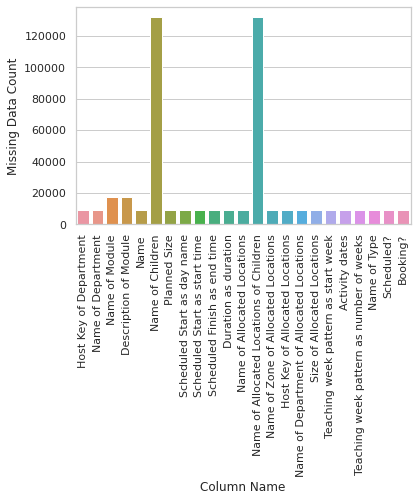
\includegraphics[width=0.5\textwidth]{resources/images/timetable data.png}
    \caption{Timetable Data}
    \label{timetable_data}
\end{figure}

From fig\ref{timetable_data},it can be inferred that almost all the columns have \textit{NaN} values but few columns have all values as \textit{NaN}. Observing data in bar charts might not provide clear understanding of the data but the data can be viewed as a percentile like shown in fig\ref{Percentage_data}.

\begin{figure}[H]
    \centering
    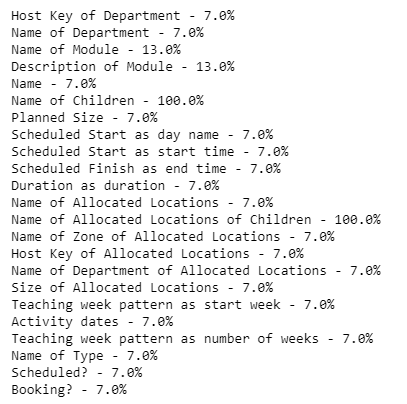
\includegraphics[width=0.5\textwidth]{resources/images/percentage data.PNG}
    \caption{Percentage Data}
    \label{Percentage_data}
\end{figure}

While cleaning the data, it is important to decide regarding the strategy for null value processing, two approaches can be used in the aforementioned case.
\begin{enumerate}
	\item Removing null values \label{app1}
	\item Setting default values to the null values\label{app2}
\end{enumerate}

Approach \ref{app1}, is not feasible because removing all the \textit{Null} values, integrity of the data would be lost.
for example, \textit{UOM-SPACE-DATA} has 1 column that has more than 90\% null values, removing these values would mean deleting 90\% of data.  To avoid data integrity issues, default values for different data-types is used. for example, \textit{string/object} data type values are assigned \textit{\_missing\_} values and \textit{Integer/Float} values are assigned \textit{0/0.0} respectively.
This means that data is not lost and can be handled in the later stages.

Once default values are set, analyse the columns that are relevant to the problem statement. If the columns are irrelevant, delete the concerned data columns. for example, \textit{Booking?} column is not related to the analysis.
Another case is excluding the unnecessary rows from the data, on observing the timetable data, it can be concluded that there exist multiple duplicate rows which can be deleted. Also, it \textit{online option} for classes and \textit{off-site} option can be excluded which are not in line with the spatial data.

Before merging the data sets, checking if all the columns match each other, if not then approximate joins are necessary. In this scenario, developing columns which are similar to the remaining data sets is achieved. for example, Timetable data set didn't had matching columns hence splitting of \textit{Host Key of Allocated Locations} and \textit{Name of Allocated Locations} and renaming the extracted data made it possible to join it with other data sets
After concluding with the preprocessing of the data, the next step would be merging the data sets. This enhances the data and assists in developing correlations between data sets. This, in turn, can be used for deducing a better model and subsequent predictions.